\documentclass{minimal}

\usepackage{tikz}

\begin{document}

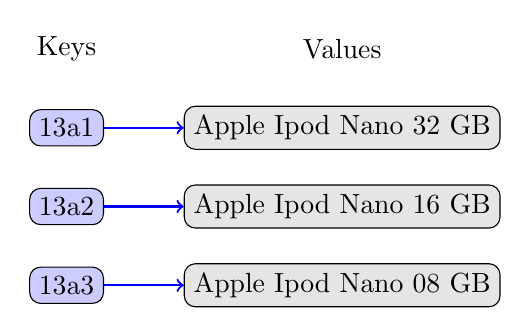
\begin{tikzpicture}

\tikzstyle{key}=[fill=blue!20, draw,rounded corners]
\tikzstyle{value}=[fill=gray!20, draw,rounded corners]
\tikzstyle{arrow}=[->, thick, blue]

\node (label_keys) {Keys};
\node [right of=label_keys, node distance=3.5cm] (label_values) {Values};

\node [key, below of=label_keys] (key1) {13a1};
\node [key, below of=key1] (key2) {13a2};
\node [key, below of=key2] (key3) {13a3};

\node [value, below of=label_values] (value1) {Apple Ipod Nano 32 GB};
\node [value, below of=value1] (value2) {Apple Ipod Nano 16 GB};
\node [value, below of=value2] (value3) {Apple Ipod Nano 08 GB};

\draw[arrow] (key1) -- (value1);
\draw[arrow] (key2) -- (value2);
\draw[arrow] (key3) -- (value3);

\end{tikzpicture}

\end{document}
